\documentclass[]{article}

\usepackage{color}
\usepackage{graphicx}
\usepackage{listings}
\usepackage[tmargin=1in,bmargin=1in,lmargin=1.25in,rmargin=1.25in]{geometry}
\usepackage{titlesec}
\titleformat*{\section}{\Large\bfseries\sffamily}
\titleformat*{\subsection}{\large\bfseries\sffamily}
\usepackage{filecontents}

\begin{filecontents}{references.bib}
@misc{dnabr,
title = {DNA baserolling: A Friday afternoon project},
author = {Jocelyne Vreede and David W. H. Swenson},
year = {2013}
}
@misc{tipsi,
title = {Transition Interface/Path Sampling Identifier},
author = {Tsjerk A. Wassenaar},
institution = {University of Amsterdam},
year = {2014}
}
@misc{gromacs,
title = {GROMACS User Manual version 4.5.4},
author = {M.J. Abraham and D. van der Spoel and E. Lindahl and B. Hess},
year = {2010}
}
@article{nikolova2011transient,
  title={Transient Hoogsteen base pairs in canonical duplex DNA},
  author={Nikolova, Evgenia N and Kim, Eunae and Wise, Abigail A and O’Brien, Patrick J and Andricioaei, Ioan and Al-Hashimi, Hashim M},
  journal={Nature},
  volume={470},
  number={7335},
  pages={498--502},
  year={2011},
  publisher={Nature Publishing Group}
}
@MISC{alaninerep,
    author = {{CP2K: Open Source Molecular Dynamics}},
    title = {Ramachandran plot for Alanine Dipeptide},
    year = {2014},
    note = {[Online; accessed July 8, 2016]},
    url = {https://www.cp2k.org/exercises:2014_ethz_mmm:alanine_dipeptide}
}
\end{filecontents}

\setlength\parindent{15pt}
\lstset{basicstyle=\ttfamily, escapeinside={\%*}{*)}}

\begin{document}

\section*{Transition Path Sampling}

\subsection*{Introduction}

Consider a molecular system that can be in two stable states, which we label as state $A$ and state $B$. An example is a protein complex, which can be in a folded or an unfolded state. To observe the way in which the system transitions from state $A$ to state $B$, we can apply Molecular Dynamics (MD) methods to simulate the system for an amount of time. Traditional MD methods can have trouble capturing a transition, however, if this transition is a \textbf{rare event}. MD simulations can be done up to an order of microseconds, which is not sufficient to capture transitions that happen at a tbeyond that timescale. This problem can be solved by performing a metadynamics simulation. For this method, we introduce a bias potential that drives the system from state $A$ to state $B$. In some cases, we can also force a transition by increasing the temperature of a traditional MD simulation, which can help proteins unfold, for example. Both these methods will provide a transition path, but not one under normal conditions. 

% Acceptatieregel in math of woorden, netjes om te noemen, niet de afleiding
If we are interested in observing the transition under normal conditions, we can apply \textbf{transition path sampling} (TPS), a rare event sampling method. TPS methods require a single transition path as an input, and can produce many new, independent ones. The input trajectory can be produced using a high temperature MD simulation, or a metadynamics simulation. TPS selects a point in this trajectory, called the 'shooting point'. From this point, then a 'shooting move' is made. In a shooting move, a new MD simulation is started, with the shooting point as a starting state. A shooting move can be backward in time or forward in time. If the simulation reaches the state ($A$ or $B$) that was reached at the corresponding end of the original parent trajectory (the front for a backward shooting move, the end for a forward shooting move), the shooting move is labelled as successful. If the shooting move is unsuccessful, it is rejected, and a new shooting move is performed. The idea is that the shooting point is chosen in such a way that the 'committor probability' is 0.5: if you start an MD simulation at this frame, there is a 50\% chance to reach both state $A$ and state $B$. A new shooting point is then picked from the trajectory of the shooting move, and the process is repeated. After several shooting moves, new paths can be constructed that go from $A$ to $B$, and are decorrelated from the original trajectory.

In this tutorial the useage of the \textsc{TIPSI} (Transition Interface/Path Sampling Identifier) package version 0.1 is demonstrated, a script that performs TPS using the \textsc{gromacs} MD engine \cite{gromacs, tipsi}. \textsc{TIPSI} is an application of rare event sampling, designed to sample many possible transition paths in a molecular system with two stable states, $A$ and $B$, where transitions between the two states are extremely rare. In this tutorial, two examples will be discussed. First, we will provide a tutorial designed to have short computational times. This tutorial concerns alanine dipeptide, and samples a transition between its two conformations. These two states are easily visually distinguishable, but the transition is not actually a rare event. The second example concerns a transition which is a rare event: the flipping of DNA basepairs from the standard Watson-Crick pairing to the non-standard Hoogsteen pairing. This transition typically does not occur even if the system is simulated for microseconds. This example uses a provided result of a metadynamics simulation as input. 

\textsc{TIPSI} relies on \textsc{GROMACS} version 4.5.4 to do molecular simulation. For this tutorial, \textsc{git} is required to pull the repository with the demonstration files. For visualizing structures, the VMD package is recommended. This tutorial is written assuming you work on a Linux system. We assume some knowledge in working with Linux, as well as a basic understanding of how to work with \textsc{GROMACS}. There will be a cheatsheet in the appendix of this tutorial for those less familiar with either. Finally, it is assumed you are working on Carbon, the clustercomputer of the Computational Chemistry group at the Universiteit van Amsterdam.
% Stukje over hoe het opgezet is naast het protocol, welk field en alles.
Both use the \texttt{TIP3P} water model. The forcefield used in the first tutorial is the \texttt{AMBER99SBILDN}, the send uses another \texttt{AMBER} forcefield included in the repository.

\subsection*{Dipeptide Alanine}

\begin{figure}[ht]
    \centering
    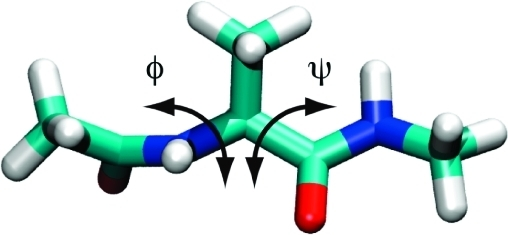
\includegraphics[width=0.5\textwidth]{images/alanine.png}
    \caption{Alanine dipeptide, dihedrals labeled $\phi$ and $\psi$, from \cite{alaninerep}.}
    \label{fig:alanine}
\end{figure}

Alanine dipeptide is a small organic molecule, consisting of the alanine amino acid with two minimal peptide bonds. This molecule has two stable states, defined by the configuration of the dihedral angles $\phi$ and $\psi$ (Fig.~\ref{fig:alanine}). In this first part of the tutorial, we will generate transition paths between the two states using \textsc{Tipsi}. To run an analysis \textsc{TIPSI}, we need to supply an intial trajectory to \textsc{TIPSI} in which the transition takes place at least once. We also need to define the stable states between which the transition takes place in a quantitative way. To get an initial trajectory, we do a preparatory MD analysis of the molecular system first.

\subsubsection*{Preparatory Analysis}

First, we log into the Carbon cluster. Make sure you are connected to the UvA network or VPN, and enter
%
\begin{lstlisting}
ssh user@carbon.science.uva.nl
\end{lstlisting}
%
When logged into the account, pull the tutorial repository to your system, which can be done by
%
\begin{lstlisting}
git clone https://github.com/dgoldsb/tipsitutorial
\end{lstlisting}
%
which will copy the tutorial directory as a new directory in your current folder. Exploring the folder shows the following subfolders:
%
\begin{lstlisting}
%*\textcolor{blue}{bin} \textcolor{blue}{documents} \textcolor{blue}{dipeptala-input} \textcolor{blue}{dnabr-input}
\newline
\textcolor{blue}{dnabr-tipsi} \textcolor{blue}{dicynebts} \textcolor{blue}{exampleresults} README.md
\end{lstlisting}
%
The folder \texttt{\textcolor{blue}{bin}} contains some analysis tools we will use later, as well as the \texttt{TIPSI} distribution. All input files required for this part of the tutorial are included in \texttt{\textcolor{blue}{dipeptala-input}}, and output will be written into a new folder \texttt{\textcolor{blue}{output}}. The \texttt{\textcolor{blue}{documents}} directory contains supporting reading material.

We enter the directory \texttt{\textcolor{blue}{dipeptala-input}} and explore, which shows the following 9 files:
%
\begin{lstlisting}
dipeptala.pdb em.mdp  emw.mdp highT.mdp md.mdp
posre.mdp submit_highT submit_md submit_tipsi
\end{lstlisting}
%
The \texttt{.pdb} file contains the structure of the molecule we simulate, in our case alanine dipeptide. To view this structure, copy the file to your own PC using a secure copy command, and view the structure in VMD. A nice piece of software that can help in copying files is FileZilla, which provides a GUI for secure copy.

To run an MD simulaton we first need to obtain the topology. We can do this by entering
%
\begin{lstlisting}
pdb2gmx -ignh -f dipeptala.pdb
\end{lstlisting}
%
picking option 6 for the \texttt{AMBER99SBILDN} forcefield, and option 1 for the \texttt{TIP3P} water model subsequently. The option \texttt{-ignh} specifies that hydroges should be ignored. Three new file should be created, namely a topology file \texttt{topol.top}, a list of atoms for a position constrained run \texttt{posre.itp}, and a set of coordinates in \textsc{Gromacs} format \texttt{conf.gro}. 

Next, we place the protein in a periodic box with a 1 nm distance between the protein and the boundary.
%
\begin{lstlisting}
editconf -f conf.gro -bt dodecahedron -d 1 -o box.gro
\end{lstlisting}
% 
We fill up the box with water molecules by running
%
\begin{lstlisting}
genbox -cs -cp box.gro -p topol.top -o solve.gro
\end{lstlisting}
%
and energy minimize this system. The settings for this MD simulation are saved in emw.mdp. Before starting the minimalization process, we combine the coordinates, topology and parameters into a \texttt{.tpr} file.
%
\begin{lstlisting}
grompp -f emw.mdp -c solve.gro -p topol.top -o emw.tpr
\end{lstlisting}
%
We run this by entering
%
\begin{lstlisting}
mdrun -deffnm emw -v
\end{lstlisting}
%
The option \texttt{-v} requests verbose output. We see that the solvent does not contain ions, thus we add 100 mM of NaCl to the system by replacing water molecules in the solvent. First, we make a new input file \texttt{ion.tpr}.
%
\begin{lstlisting}
grompp -f emw.mdp -c emw.gro -p topol.top -o ion.tpr
\end{lstlisting}
%
We add ions to this as follows
%
\begin{lstlisting}
genion -s ion.tpr -p topol.top -neutral -conc 0.1 -o ion.gro
\end{lstlisting}
%
We pick option 13 to replace water molecules with Na$^+$ and Cl$^{-1}$ ions. For a system this small, only one or several of each will be added. We now energy minimize the system again.
%
\begin{lstlisting}
grompp -f em.mdp -c ion.gro -p topol.top -o em.tpr
mdrun -deffnm em -v
\end{lstlisting}
% 
To relax the water and ions around the protein we perform a position constrained run. This implies that all non-hydrogen atoms in the protein are fixed in their position.
%
\begin{lstlisting}
grompp -f posre.mdp -c em.gro -p topol.top -o posre.tpr
mdrun -deffnm posre -v
\end{lstlisting}
%
To visualize the trajectory later, we need to make a snapshot of the system at the start of the MD simulation. IN order to do so, we run
%
\begin{lstlisting}
trjconv -f posre.gro -s posre.tpr -pbc mol -center  -ur compact -o dipept_show.gro
\end{lstlisting}
%
We pick option 1 for our first option to center the protein. The second option depends on your hardware and the length of your simulation. In this case we can pick option 0, as the system is small. If your simulation is long, the system is big, or your RAM is limited, option 1 is preferred to ignore solvent molecules. The output \texttt{dipept\_show.gro} can be visualized in \textsc{VMD}.

%Already added solvent, did an energy minimization and contrained run. 
Now that we have relaxed the solvent we can run an MD simulation. We want to ensure that the transition between the two states takes place, so it is typically not a bad idea to run at a higher temperature (400K). The resulting trajectory will serve as an input for \textsc{TIPSI}, and will be used to find many more transitions.
%
\begin{lstlisting}
grompp -f highT.mdp -c posre.gro -p topol.top -o highT.tpr
qsub submit_highT
\end{lstlisting}
%
We will also run the simulation at room temperature, but for a shorter duration, in order to define the stable states. The\texttt{.tpr} file in which the MD simulation conditions that you are interested in are defined is also an input for \textsc{tipsi}. These conditions will be used for all simulation run in the TPS process. We want these simulations to take place at room temperature (298K). We generate the \texttt{.tpr} and run the simulation as follows:
%
\begin{lstlisting}
grompp -f md.mdp -c posre.gro -p topol.top -o md.tpr
qsub submit_md
\end{lstlisting}
%
The output will be put in the \texttt{\textcolor{blue}{output}} directory.

\subsubsection*{Running TIPSI}

Before all else, we should check if the right files are flagged as executable. The file \texttt{/documents/executables.txt} contains a list of all files in the \texttt{/bin/tipsi/}-directory that should be flagged as executable. Executable files should show green when using the \texttt{ls} command in this directory. Making files executable is done with \texttt{chmod +x file}.

To tell \textsc{TIPSI} how to define the stable states, we have to set up a parameter (\texttt{.par}) file. To find if there are stables states between which a transition can take place, we need to express our trajectory in terms of some collective variable. In this example, we use two dihedrals, $\phi$ and $\psi$. We create a an index file defining these dihedrals by going to the output directory of the room temperature simulation, and run
%
\begin{lstlisting}
vim angle.ndx
\end{lstlisting}
%
after which we copy-paste the following:
%
\begin{lstlisting}
[ Phi ]
5 7 9 15

[ Psi ]
7 9 15 17
\end{lstlisting}
%
After we save and quit (\texttt{:wq} in vim), we analyze our simulation using the dihedrals describedz in the index file. We run
%
\begin{lstlisting}
g_angle -f md.xtc -od angle.ndx -ov dihed_phi.xvg -type dihedral
\end{lstlisting}
%
with option 0 and 
%
\begin{lstlisting}
g_angle -f md.xtc -od angle.ndx -ov dihed_psi.xvg -type dihedral
\end{lstlisting}
%
with option 1 to generate a dataset of the dihedral angles. We can visualize how often each combination of these two variables is visited by running
%
\begin{lstlisting}
python ../../bin/generate2Dbins.py dihed_phi.xvg 1 dihed_psi.xvg 
1 -180 180 -180 180 100 100 Phi Psi Dihedrals\ Landscape
\end{lstlisting}
%
This script will generate a set of plots in \texttt{.pdf} format. Transfer the plots to your computer and view them. You will see that there are two combinations of the dihedral angles that are visited a lot by the simulation. We see that the area between these two states are not visited often. As such, they can be considered semi-stable, and are our A and B state for \textsc{TIPSI}. Note down the ranges for both variables at which the molecule is in a semi-stable state. Be sure that the system does not go outside this range while still being in the stable configuration, as this is problematic for \textsc{tipsi}.

Go to the \textcolor{blue}{\texttt{bin}} directory, and look at the \texttt{tps-dipept.par} file. In this file, we define the maximum length of a transition path, as well as when the system is in state A, state B, or inbetween (I). Confirm that we confirmed the state in accordance with the range that you noted down. There is little documentation so far on how to include other variables in the parameter file, so some alternative options are included in an appendix.

We included groups of atoms in out parameter file, namely \texttt{phi} and \texttt{psi}. We must define this custom group in an \texttt{.ndx} file to pass this group to TIPSI. If explore the \textcolor{green}{\texttt{run\_tipsi-dipept}} file, we see that the \texttt{angle.ndx} file is taken as input. To make sure that this file is copied to the node, we make a copy of the file in the \textcolor{blue}{\texttt{dipeptala-input}} directory. In \textcolor{green}{\texttt{run\_tipsi-dipept}} , we can also set the number of processors used by \textsc{tipsi}, which should match the number we assigned in the submit script (8 processors), as well as the number of shooting moves performed, which in this case is set to 10. As a sidenote, by generating an index file with \textsc{gromacs}, you can use any of the \textsc{gromacs} standard groups. 

Finally, we need to copy our initial trajectory to our input directory. Change your directory to your high temperature MD output, and exectute 
%
\begin{lstlisting}
cp highT.trr ../../input-dipeptala/highT.trr
\end{lstlisting}
%

Now that we set up the parameter file, we need to edit our run script to take the correct input. Open the file \textcolor{green}{\texttt{run\_ tipsi-dipept}}, and check if the \texttt{.tpr} file (for the simulation setting) and the \texttt{.trr} file (for the trajectory) are set correctly. Run \textsc{TIPSI} by entering
%
\begin{lstlisting}
qsub submit_tipsi
\end{lstlisting}
%

\subsubsection*{Analyzing Results from TIPSI}

Running \textsc{tipsi} takes some time. While it runs, go to the directory \textcolor{blue}{\texttt{exampleresults/DATA}}. This folder contains some output generated in \textsc{tipsi}, bar the output trajectories. Explore the directory, you should see
%
\begin{lstlisting}
0 1 2
\end{lstlisting}
%
This implies that three shooting moves have been done. Now go to the directory \textcolor{blue}{\texttt{0/0}}, and do
%
\begin{lstlisting}
more 0-0.dat
\end{lstlisting}
%
Can you confirm that a transition took place? Now move up two directories, and go to the directory \textcolor{blue}{\texttt{2}}. Explore this directory, you should see
%
\begin{lstlisting}
0 1
\end{lstlisting}
%
This means there have been two attempts at a shooting move until one was accepted. Move to the directory \textcolor{blue}{\texttt{0}}, and execute
%
\begin{lstlisting}
more 2-0-FW.dat
\end{lstlisting}
%
This is a forward shooting move, as indicated by \texttt{FW}, and thus advances in time. Can you see why this shooting move was not accepted? Finally, move up one directory, and go to the directory \textcolor{blue}{\texttt{1}}. This is a backward trajectory, as indicated by the \texttt{BW} flag. Execute
%
\begin{lstlisting}
more 2-1-BW.dat
\end{lstlisting}
%
\textsc{TIPSI} does backward shooting moves by taking a negative timestep, can you confirm this? Can you see why this trajectory was accepted? The total trajectory, if accepted, is also described in a \texttt{dat} file. Execute
%
\begin{lstlisting}
more 2-1.dat
\end{lstlisting}
%
Can you identify which parts of the trajectory come from which shooting move?

The \textcolor{green}{\texttt{bin/match\_paths.sh}} script should put together all the trajectories automatically before the output is copied from the node to you own directory. All paths can be found in the \textcolor{blue}{\texttt{output/jobname/DATA}} directory. Copy a complete trajectory to your own PC to confirm that the trajectory is correct, by visualizing it in \textsc{VMD}. You can compare your result to the trajectory in the \textcolor{blue}{\texttt{exampleresults}} folder.

The \textcolor{green}{\texttt{bin/match\_paths.sh}} script also output a file that contains some data on the TPS process. We can process this information by running
%
\begin{lstlisting}
python ../../../bin/processTIPSImerge.py metainfo.csv
\end{lstlisting}
% 
This has to be done on your own machine, however, as an image is outputted to the screen, and Carbon runs outdated Python libraries. The output will detail the average path length of the accepted paths, number of decorrelated paths, the shooting tree, and the ratio between forward shooting moves and backward shooting moves. Did the shooting process take place as you had expected? If you feel brave, you can check if there were no warnings or errors by opening \texttt{mergelog.txt} and searching for WARNING/Warning/warning and error. 

\newpage

\subsection*{DNA Baseroll}

\begin{figure}[ht]
    \centering
    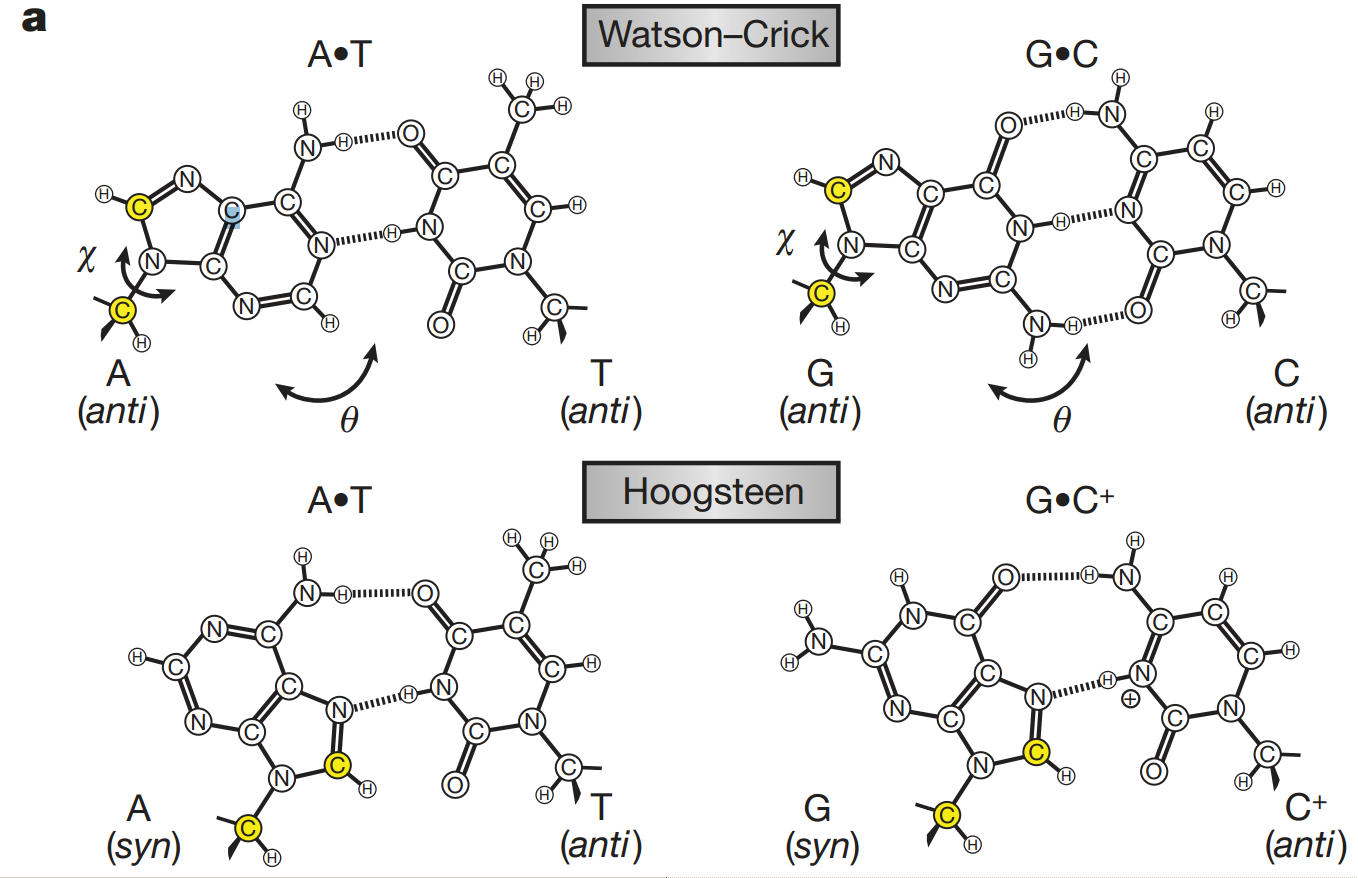
\includegraphics[scale=0.25]{images/pairing.png}
    \caption{Hoogsteen and Watson-Crick pairing, from \cite{nikolova2011transient}.}
    \label{fig:dnabr}
\end{figure}

For the second example, we examine the case of the 'DNA baseroll', based on a project by Jocelyne Vreede and David Swenson (the original presentation is included in the \texttt{\textcolor{blue}{documents}} directory) \cite{dnabr}. This is an actual rare event, in which a DNA basepair transition from the Watson-Crick configuration to the Hoogsteen pairing, or vice versa. These two configurations are illustrated in Fig.~\ref{fig:dnabr}. This event typically does not occur when running a normal MD simulation for a microsecond, but using \textsc{tipsi} we will generate several new transitions.

\subsubsection*{Preparation}

We again log into the Carbon cluster. Make sure you are connected to the UvA network or VPN, and enter
%
\begin{lstlisting}
ssh user@carbon.science.uva.nl
\end{lstlisting}
%

We enter the directory \texttt{\textcolor{blue}{dna-br}} and explore, which shows the following files:
%
\begin{lstlisting}
conf.gro run.mdp submit_md topol_DNA_chain_A.itp 
topol_DNA_chain_B.itp topol_DNA.itp topol_Ion2.itp topol.top %*\textcolor{blue}{top}
\end{lstlisting}
%
First, we need to install a custom topology, which we do by running
%
\begin{lstlisting}
export GMXLIB=./top
\end{lstlisting}
%
We can generate the \texttt{tpr} file necessary to run \textsc{tipsi} by executing
%
\begin{lstlisting}
grompp -f run.mdp -c conf.gro -p topol.top -o md.tpr
\end{lstlisting}
%
after which we move this file to our directory for \textsc{tipsi} input
%
\begin{lstlisting}
mv md.tpr ../dnabr-tipsi/
\end{lstlisting}
%
Normally it is necessary to run a regular MD simulation to confirm that the two states are stable, but in this example this is a given. This can still be done by running the submit script, if you are interested in confirming that the transition does not happen at room temperature in a regular MD simulation.

\subsubsection*{Running TIPSI}

To tell \textsc{TIPSI} how to define the stable states, we have to set up a parameter (\texttt{.par}) file. The stable states are in this case define by whether certain hydrogen bonds exist. In Fig.~\ref{fig:dnabr}, we can see the hydrogen bonds formed in both pairings. We are dealing with an A-T basepair, so there should be two hydrogen bonds in either configuration. One hydrogen bond is always present, and is between atoms 275 and 492. The hydrogen bond unique in the Watson-Crick pairing is between atoms 276 and 495, and the bond unique to the Hoogsteen pairing is between 276 and 289.

Go to the \textcolor{blue}{\texttt{bin}} directory, and look at the \texttt{tps-dnabr.par} file. In this file, we define the maximum length of a transition path, as well as when the system is in state A, state B, or inbetween (I). Confirm that we confirmed the state correctly. Notice that the numbers are not the same! This is because we define the atoms now in a Numpy array. This array is 0-indexed, whereas \textsc{gromacs} starts counting at 1. For more information on this, read the appendix on \textsc{tipsi} parameter files.

Now that we set up the parameter file, we need to edit our run script to take the correct input. Open the file \textcolor{green}{\texttt{run\_tipsi-dnabr}}, and check if the \texttt{.tpr} file (for the simulation setting) and the \texttt{.trr} file (for the trajectory) are set correctly. Run \textsc{TIPSI} by entering
%
\begin{lstlisting}
qsub submit_tipsi
\end{lstlisting}
%
in the \textcolor{blue}{\texttt{dnabr-tipsi}} directory.

\subsubsection*{Analyzing Results from TIPSI}

As in the previous example, you should compare your result to the transition in the \textcolor{blue}{\texttt{exampleresults}} folder to verify that you captured the transition. The basepair of interest can be isolated in \textsc{VMD} by visualizing only \texttt{resname DT and resid 9}, and \texttt{resname DA and resid 4}. If you use the RMSD trajectory tool in VMD, make sure to change 'protein' to 'nucleic' before hitting 'ALIGN'. You can process the information in the TPS process again by running
%
\begin{lstlisting}
python ../../../bin/processTIPSImerge.py metainfo.csv
\end{lstlisting}
% 
on your PC. Is the ratio between backward and forward shooting moves about 0.5? And is the tree similarly shaped as the tree from example 1?

\bibliographystyle{plain}
\bibliography{references}

\newpage

\appendix
\section*{Linux Cheatsheet}
\setlength\parindent{0pt}

\begin{itemize}
\item \textbf{Display current directory}: \texttt{pwd}

\item \textbf{View contents of the current directory}: \texttt{ls}

\item \textbf{Change the directory}: \texttt{cd ./your/directory/here}

\textbf{Note}: the currect directory is referred to as \texttt{./}, the directory in which your current directory resides is \texttt{../}

\item \textbf{Copy a directory/file}: \texttt{cp ./target ./new/location/}

\textbf{Note}: the option \texttt{-r} (recursive) is required for directories, this implies all the contents should be copied

\item \textbf{Delete a directory/file}: \texttt{rm ./target}

\textbf{Note}: again the recursive option is required for directories, and mind that deleted directories cannot be recovered.

\item \textbf{Read a file}: \texttt{more ./target} or \texttt{head ./target} or \texttt{tail ./target}

\item \textbf{Make a file executable}: \texttt{chmod +x ./target}
\end{itemize}

\newpage
\section*{GROMACS Cheatsheet}

\begin{itemize}
\item \textbf{Check the temperature of a simulation}: \begin{verbatim}gmxdump -s target.md | grep ref_t\end{verbatim}
\item \textbf{Check aspects of a trajectory}: \begin{verbatim}gmxcheck -f target.trr | more\end{verbatim}
\item \textbf{Add a forcefield (for DNA baseroll)}: \begin{verbatim}export GMXLIB=./top\end{verbatim}
\item \textbf{Obtain a centere \texttt{.gro} of the system}: \begin{verbatim}trjconv -f target.gro -s target.tpr -pbc mol -center -ur compact -o output.gro\end{verbatim}
\item \textbf{Convert a \texttt{.trr} to a \texttt{.xtc}}: \begin{verbatim}trjconv -f target.xtc -s target.tpr -pbc mol -center -ur compact -o ouput.xtc\end{verbatim}
\item \textbf{List distance between two atoms or center of mass}: \begin{verbatim}g_dist -f target.trr -s target.tpr -n index.ndx -o pdist.xvg\end{verbatim}
\item \textbf{List the RMSD}: \begin{verbatim}g_ -f target.xtc -s target.tpr -o rmsd.xvg;
1; 1\end{verbatim}
\item \textbf{List the free energy}: \begin{verbatim}g_energy -f target.edr -o free_energy.xvg\end{verbatim}
\item \textbf{List the number of helical hydrogen bonds}: \begin{verbatim}g_hbond -f target.xtc -s target.tpr -hx hbhelix.xvg; cat hbhelix.xvg | grep -v "^\#"| grep -v "^\@" | awk '{print $1"  "$6}' > output.xvg\end{verbatim}
\item \textbf{Track a dihedral}: \begin{verbatim}mk_angndx -s target.tpr -n angle.ndx -type dihedral; g_angle -f target.xtc -od angles.ndx -n dihed.xvg -type dihedral\end{verbatim}
\item \textbf{List radius of gyration}: \begin{verbatim}g_gyrate -f target.xtc -s target.tpr -o gyrate.xvg\end{verbatim}
\end{itemize}

\newpage
\section*{TIPSI Cheatsheet}

\subsection*{Running parameters}

In general, we run \textsc{tipsi} using the \texttt{run tipsi}-script included in the \textcolor{blue}{\texttt{./bin/tipsi/calculator}}-directory. 
Examining this script reveals that \textsc{tipsi} takes the following input parameters in the case of this tutorial:

\begin{lstlisting}
./tipsi/tipsi.sh -v -tpr md.tpr -trr 000003.trr -par tps.par 
-ndx index.ndx -maxc 10 -np 16 -mdrun "\$MDRUN"
-gmxrc "/share/apps/gromacs/openmpi-intel/gromacs-4.5.4/bin/GMXRC" 
\end{lstlisting}

The parameter \texttt{-v} enables verbose output, which is written to the \texttt{O}-file in the output directory. 
In general this is helpful, as it will give some indication of where things go wrong when a run fails. 
The MD-settings are then read from a tpr-file, entered under \texttt{-tpr}. 
The initial trajectory is loaded in with \texttt{-trr}. 
The parameter file is loaded in with \texttt{-par}, and the groups that are used in the parameter file with \texttt{-ndx}. 
The number of processors for MPI is set with \texttt{-np}. 
The number of shooting moves performed is set with \texttt{-maxc}.
Finally, the correct \textsc{gromacs} executables are linked to with \texttt{-gmxrx} and \texttt{-mdrun}.
Additional parameters can be found by running \textsc{tipsi} with the \texttt{-h} command.

\subsection*{Making a .par file}

A paremeter file contains several pieces of information. First, the maximum frames of a trajectory is defined. 
Second, the groups have to be defined, as well as the parameters. 
For the parameter definitions, a number of functions in \textsc{tipsi} can be used. 
Many have a corresponding function native to \texttt{gromacs} that provides the same output. 
A list of all functions, and their parameters, will be provided in this appendix. 
Third, we have to define the states of the system using these parameters.
The states are a boolean expression, written in Python-syntax. An example is:

\begin{lstlisting}
state A = (0.25 < wc & wc < 0.35 & 0.38 < hg)
state B = (0.25 < hg & hg < 0.35 & 0.38 < wc)

interface I = (!A) & (!B)
\end{lstlisting}

It is noteworthy that \textsc{tipsi} seems to not handle excessive brackets well, so try to keep your statement within a single pair of brackets, and use the priority order of different operators to your advantage.
The intermediate state is always defined as not A and not B. If no states are defined, the order parameters will be calculated for every frame. This can be useful to determine the states, as \textsc{gromacs} in some cases does not calculate the order parameters in the same way as \textsc{tipsi}.
Finally, the parameter file is finished with a set of recrossing rules. These are generally kept the same.

\subsection*{Defining groups}

In general, the way to specify a group of atoms in \textsc{tipsi} is through a numpy array. 
For example, we can find the radius of gyration of atom 5, 7, 13 and 18 through:

\begin{lstlisting}
init group = numpy.array((5, 7, 13, 18))
par rg  = rgyration(frame[acc,:])
\end{lstlisting}

Groups can be specified in an index file, which has to be included as a parameter. 
A standard index file, as generated by \texttt{gromacs}, contains a number of standard groups. 
These include the entire protein, the carbon backbone, and the sidechains. For example, we can find the radius of gyration over the entire protein:

\begin{lstlisting}
par rg  = rgyration(frame$Protein)
\end{lstlisting}

\textsc{Tipsi} is often flexible when it comes to defining pairs. For example, the calculater function that calculates the periodic distance between two atoms can take both two seperate atoms as an input, as well as on numpy array of two atoms. This is demonstrated below:

\begin{lstlisting}
par dist1 = pdist(frame[5,:],frame[7,:])

init pair = numpy.array((5, 7))
par dist2 = pdist(frame[pair,:]) 
\end{lstlisting}

\textbf{IMPORTANT NOTE}: \textsc{tipsi} starts its index with 0, whereas \textsc{gromacs} starts with 1. To avoid off-by-one errors, make sure you subtract 1 off every atom number when you write them directly into the parameter file. The index files read into \textsc{tipsi} are 1-indexed, however, so \texttt{ndx} files do not have to be altered.

\subsection*{Calculator options}

Below, we show a list of the available functions to define parameters in the .par file. An atom or group of atoms is always defined within a frame. 
Each frame is a $n \times 3$ array, containing the x/y/z-coordinates of all $n$ atoms in the trajectory. 
Some functions can take weights as an input argument. For example, the atom mass can be use as a weight in many cases.
The weights can be extracted from, for example, the \texttt{.itp}-files in the example.
The weights can be loaded into \texttt{tipsi} by including them as a numpy-array in the parameter file. 
If a periodic version exists, \texttt{box} as an argument. Non-periodic conditions are assumened if \texttt{box} is left as \texttt{none}.
Alternatively, the list can be included in the index-file, as groups in the index files are simply loaded as arrays.
A final important note that for distances, it is preferable to input two of the same atoms at once, so \texttt{frame[numpy.array((1,1)),:]}, and adding \texttt{.min()} after the command.
This is because some distance functions need an array input for the atom numbers, regardless of whether it is only one atom.
For more information, explore \texttt{functions.py} in the \textcolor{blue}{\texttt{./bin/tipsi/calculator}} folder.

\begin{itemize}
\item 	\texttt{com(coord, box, weights)}\\
		\textbf{Center of Mass}: mass of a set of atom numbers \texttt{coord} (numpy array or index group).
\item 	\texttt{dist(a, b, box, what)}\\
		\textbf{Distance}: the distance between atom numbers \texttt{a} and \texttt{b}. The mode \texttt{what} can be set to Euclidean or Manhattan.
\item 	\texttt{angle(a, b, c)}\\
		\textbf{Angle}: the angle between atom numbers \texttt{a}, \texttt{b} and \texttt{c}.
\item 	\texttt{dihrad(a, b, c, d)}\\
		\textbf{Dihedral (radians)}: the dihedral between atom numbers \texttt{a}, \texttt{b}, \texttt{c} and \texttt{d} in radians.
\item 	\texttt{dihdeg(a, b, c, d)}\\
		\textbf{Dihedral (degrees)}: the dihedral between atom numbers \texttt{a}, \texttt{b}, \texttt{c} and \texttt{d} in degrees.
\item 	\texttt{rgyr(x)}\\
		\textbf{Radius of gyration}: the radius of gyration over a set of atom numbers \texttt{x}.
		It should be noted that, unlike in \textsc{gromacs}, this is not standard weighted with the atom mass.
\item 	\texttt{rmsd(x, y)}\\
		\textbf{Root-mean-square-deviation}: the RMSD between the groups of atom numbers \texttt{x} and \texttt{y}.
\item 	\texttt{hbonds(D, H, A, mode, box)}\\
		\textbf{Hydrogen bonds}: returns the number of hydrogen bonds between a group of donors (an array of atom numbers \texttt{D}), hydrogens (an array of atom numbers \\texttt{H}) and acceptors (an array of atom numbers \texttt{A}). The \texttt{mode} can be set to \texttt{dha}, in which case only triplets are considered in the order given. If not, then all possible combinations of donors, hydrogens and acceptors are considered. 
\end{itemize}

\end{document}